\clearpage

\subsection{文字を表示する命令}

LEDがてんめつしている間、画面には「OK!」のメッセージが表示されています。

\begin{figure}[H]
    \begin{center}
        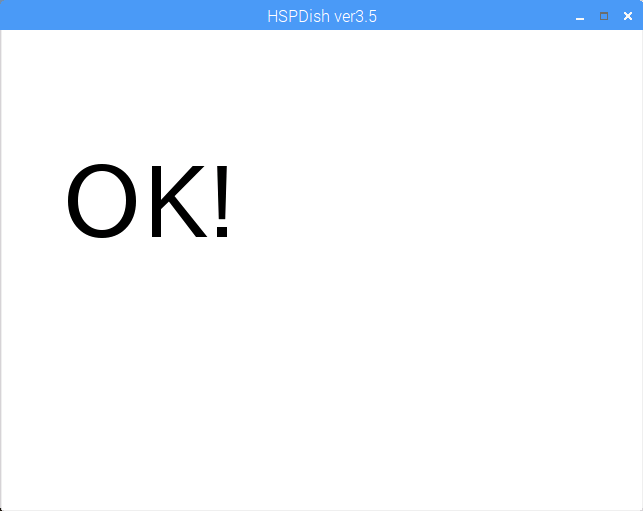
\includegraphics[keepaspectratio,width=5.741cm,height=4.572cm]{text02-img/text02-img027.png}
        \caption{OK!のメッセージ}
    \end{center}
\end{figure}

実行されているスクリプトを見てみましょう。
「mes “OK!”」と書かれている行が関係ありそうですね。
ためしに{\textquotedbl}OK!{\textquotedbl}のかわりに自分の名前を入れてみましょう。

\begin{description}
    \item mes {\textquotedbl}takeda{\textquotedbl}
\end{description}

打ち込んだら[F5]を押してちゃんと動くか見てみましょう。

\begin{description}
    \item (HSPのルール)
\end{description}

\begin{description}
    \item mes命令は文字を画面に出す命令
    \item mesの後にスペースに続けて表示したい文字を指定します
    \item 必ず「{\textquotedbl}」で文字を囲むこと
\end{description}

mesという命令で文字を出すことができます。今度はパラメーターに「”」の記号で囲んだ文字を使っています。パラメーターで指定する時は、「”」で囲んだ文字か、数字になることを覚えておきましょう。

このようにコンピューターにわかる言葉、スクリプトを正しく書くことで、その通りに動いてくれます。
どんなに間違ったとしてもコンピューターがこわれることはありません。
HSPのルールを守らないとエラーが表示されてしまいます。
ターミナルの画面に、何行目でエラーが出たのかが表示されるので、その行を見直すといいでしょう。